%% 
%% 4. Vorlesung <2012-10-26 Fri>
%% 
%% Skript Differentialgeometrie im Wintersemester 12/13
%% Zur Vorlesung von Dr. Grensing am KIT Karlsruhe
%% 
%% Mitschrieb und Textsatz von Jan-Bernhard Kordaß.
%% 

\chapter{Differentiale}
Es seien $M$ und $N$ glatte Mannigfaltigkeiten und $\Phi \colon M \to N$ eine glatte Abbildung.
Sind $p \in M$ und $X_p \in \T_pM$ , so ist 
\begin{align*}
	\Phi_{*p}X_p \colon C^{\infty}(N) \to \R, f \mapsto X_p(\underbrace{f \circ \Phi}_{\in C^{\infty}(N)}).
\end{align*}
ein Tangentialvektor an $N$ in $\Phi(p)$:
\begin{align*}
	\Phi_{*p}X_p(fg) & = X_p((f \circ \Phi)(g \circ \Phi)) = X_p(f \circ \Phi)(g \circ \Phi)(p) + (f \circ \Phi)(p)X_p(g \circ \Phi)\\
	& = \Phi_{*p}X_p(f)\textcolor{red}{g}(\Phi(p)) + f(\Phi(p)) \Phi_{*p}X_p(g).
\end{align*}
\begin{center}\begin{tikzpicture}[font=\scriptsize]
    % \draw[step=0.25,gray!15] (-6,-1) grid (6,5); \draw[step=0.5,gray!30] (-6,-1) grid (6,5); \fill (0,0) circle(0.1); %Hilfsgitter
    
    % Die Abbildungspfeile
    \draw[->] (-1.5,0) to[out=20, in=160]node[above]{$\psi' \circ \Phi \circ \varphi^{-1}$}node[below]{diff'bar} (1.5,0);
    \draw[->] (-1.5,3) to[out=20, in=160]node[above]{$\Phi$} (1.5,3);
    
    % Die Achsen
    \draw[->,thick] (-5.5,-0.5) -- (-2,-0.5); \draw[->,thick] (-5.25,-0.75) -- (-5.25, 1.25); \node[font=\normalfont] at (-2,1.25) {$\R^m$};
    \draw[->,thick] (2,-0.5) -- (5.5,-0.5); \draw[->,thick] (2.25,-0.75) -- (2.25, 1.25); \node[font=\normalfont] at (5.5,1.25) {$\R^n$};
    
    % das linke Ding
    \coordinate (ding0) at (-3.5,4.5); \coordinate (ding1) at (-4.25,3.5); \coordinate (ding2) at (-4.5,2); \coordinate (ding3) at (-2.75,2.5); \coordinate (ding4) at (-1.5,4);
    \coordinate (ctrld0) at (0.5,-0.25); \coordinate (ctrld1) at (0.75,0.5); \coordinate (ctrld2) at (-0.5,0.5); \coordinate (ctrld3) at (0.25,0.5); \coordinate (ctrld4) at (-0.75,0); 
    \draw[thick] (ding0) ..controls($(ding0)+(ctrld0)$) and ($(ding1)+(0.75,0.5)$).. (ding1) ..controls($(ding1)-(ctrld1)$) and($(ding2)+(ctrld2)$).. (ding2) ..controls($(ding2)-(ctrld2)$) and ($(ding3)-2*(ctrld3)$).. (ding3) ..controls($(ding3)+(ctrld3)$) and ($(ding4)+(ctrld4)$).. (ding4);
    % das Loch in der Mitte nicht vergessen, es besteht aus zwei geclipten Kreisen
    \begin{scope}
      \clip (-4.25,2.5) rectangle (-2.75,3);
      % \draw[thick] (-4.25,3) to[out=330,in=180] (-3.5,2.75) to[out=0,in=210] (-2.75,3);
      \path[draw,thick,name path=gkreis] (-3.5,4.25) circle (1.5);
    \end{scope}
    \path[name path=kkreis] (-3.5,2) circle(1);
    \path[name intersections={of=gkreis and kkreis}];
    \begin{scope}
      \clip (intersection-1) rectangle ($(intersection-2)+(0,0.5)$);
      \draw[thick]  (-3.5,2) circle(1);
    \end{scope}
    
    % das rechte Ding
    \draw[thick] (4, 3)  ellipse (2 and 1);
    % und das Loch
    \begin{scope}
      \clip (3, 2.75) rectangle (5, 4);
      \path[draw,thick,name path=gkreis] (4,3.75) ellipse (1.25 and 1);
    \end{scope}
    \path[name path=kkreis] (4,2.5) ellipse (1 and 0.75);
    \path[name intersections={of=gkreis and kkreis}];
    \begin{scope}
      \clip (intersection-1) rectangle ($(intersection-2)+(0,0.5)$);
      \draw[thick] (4,2.5) ellipse (1 and 0.75);
    \end{scope}
    
    % die linke Kartoffel
    \coordinate (kartoffel0) at (-4.25,2.5); \coordinate (kartoffel1) at (-4.25,2); \coordinate (kartoffel2) at (-4,2.125); \coordinate (kartoffel3) at (-3.75,2); \coordinate (kartoffel4) at (-3.25,2.5); \coordinate (kartoffel5) at (-3.75,2.5); 
    \coordinate (ctrlk0) at (0.25,0.25); \coordinate (ctrlk1235) at (0.25,0); \coordinate (ctrlk4) at (0,0.25);
    \draw (kartoffel0) ..controls($(kartoffel0)-(ctrlk0)$) and ($(kartoffel1)-0.5*(ctrlk1235)$).. (kartoffel1) ..controls($(kartoffel1)+0.5*(ctrlk1235)$) and ($(kartoffel2)-(ctrlk1235)$).. (kartoffel2) ..controls($(kartoffel2)+(ctrlk1235)$) and ($(kartoffel3)-0.5*(ctrlk1235)$).. (kartoffel3) ..controls($(kartoffel3)+2*(ctrlk1235)$) and ($(kartoffel4)-(ctrlk4)$).. (kartoffel4) ..controls($(kartoffel4)+(ctrlk4)$) and ($(kartoffel5)+(ctrlk1235)$).. (kartoffel5) ..controls($(kartoffel5)-0.5*(ctrlk1235)$) and ($(kartoffel0)+(ctrlk0)$).. (kartoffel0) -- cycle;
    \fill (-3.75,2.25) circle (0.05) node[right]{$p$};
    
    % die rechte Kartoffel (Kreis)
    \draw (4,2.5) ellipse (0.5 and 0.25); \fill (4,2.5) circle (0.05) node[right]{$q$};
    
    % die beiden Umgebungen unten
    \draw (-3.75,0.25) circle (0.5); \fill (-3.75,0.25) circle (0.05) node[right]{$x$};
    \draw (4,0.25) circle (0.5); \fill (4,0.25) circle (0.05) node[right]{$y$};
    
    % Abbildungspfeile
    \draw[->] (-4, 2.25) to[out=250,in=110] node[left]{$\varphi$} (-4,0.75);
    \draw[->] (3.75, 2.5) to[out=250,in=110] node[left]{$\psi$} (3.75,0.75);
  \end{tikzpicture}\end{center}

% Definition 3.1
\begin{Dfn}
  Die lineare Abbildung $\Phi_{*p} \colon \T_pM \to \T_{\Phi(p)}N$ heißt das \CmMark{Differential} von $\Phi$ in $p$. Der Rang von $\Phi_{*p}$ bezeichnet man als den Rang von $\Phi$ in $p$.
\end{Dfn}

% Lemma 3.2
\begin{Lemma}[Differentiale in lokalen Koordinaten]
  Sind $\varphi$ und $\psi$ Karten von $M$ und $N$ um $p$ und $\Phi(p) = q$, sowie $\pdifffrac[p]{}{x^i}$ und $\pdifffrac[q]{}{y^i}$ die Standardbasen von $\T_pM$ und $\T_qN$ bezüglich der Karten $\varphi$ und $\psi$, so gilt:
  \begin{align*}
    \Phi_{*p}\pdifffrac[p]{}{x^i} = \sum \partial_i\left(\psi^j \circ \Phi \circ \varphi^{-1}\right)\big(\varphi(p)\big)\pdifffrac[q]{}{y^j}.
  \end{align*}
  Die partielle Ableitung $\partial_i(\psi^j \circ \Phi \circ \varphi^{-1})(\varphi(p))$ bezeichnet man auch kurz $\frac{\partial \Phi^j}{\partial x^i}(p)$.
\end{Lemma}

\begin{Bem}
  Aus der Linearität von $\Phi_{*p}$ folgt, dass für $X_p = \sum \xi^i\pdifffrac[p]{}{x^i} \in \T_pM$ und $\Phi_{*p}X_p = \sum \eta^j\pdifffrac[q]{}{y^j}$ gilt:
  \begin{align*}
    \eta^j = \sum \frac{\partial \Phi^j}{\partial x^i}\xi^i \text{, beziehungsweise } \eta = \D(\psi \circ \Phi \circ \varphi^{-1})\xi.
  \end{align*}
\end{Bem}

\begin{proof}
  \begin{align*}
    \underbrace{\left(\Phi_{*p}\pdifffrac[p]{}{x^i}\right)}_{\textcolor{red}{\in \T_qN}}(\psi^j) = \pdifffrac[p]{}{x^i}(\psi^j \circ \Phi) = \partial_i (\psi^j \circ \Phi \circ \varphi^{-1})(\varphi(p)) = \frac{\partial \Phi^j}{\partial y^i}(p).
  \end{align*}
\end{proof}

\begin{Bem}[Charakterisierung durch Kurven]
  Ist $[c] \in \T_p\textcolor{red}{M}$, so gilt für $f \in C^{\infty}(\textcolor{red}{N})$:
  \begin{align*}
    \Phi_{*p}[c](f) = [c](f \circ \Phi) = \difffrac[t=0]{}{t}(\underbrace{f \circ \Phi \circ c)}_{\substack{\text{glatte Kurve}\\ \text{auf }N}} = [\Phi \circ c](f)
  \end{align*}
  also $\Phi_{*p}[c] = [\Phi \circ c]$.
\end{Bem}

\begin{Bem}[Tangentialräume an Untermannigfaltigkeiten des $\R^n$]
  \marginnote{\begin{tikzpicture}
	%\draw[step=0.25,gray!15] (-6,-5) grid (6,3); \draw[step=0.5,gray!30] (-6,-5) grid (6,3); \fill (0,0) circle(0.1); %Hilfsgitter
	\draw[->] (-0.5,0) -- (2.75,0); \draw[->] (0,-0.5) -- (0,2); \draw[->] (-0.5,-0.25) -- (2,1);
	\draw[->] (-0.5,-3) -- (2.75,-3) node[above]{$\R^m$}; \draw[->] (0,-3.5) -- (0,-1);
	\draw (1.75,-2) circle (0.5); \node at (1,-1.5) {$U$};
	%Segel
	\coordinate (segel1) at (0.25,1.25); \coordinate (segel2) at (3,2.25); \coordinate (segel3) at (2.25,1);
	\coordinate (ctrl1) at (0.5,0.75); \coordinate (ctrl2) at (-1,0.25); \coordinate (ctrl3) at (-0.5,-0.5); \coordinate (ctrl4) at (0.25,0.5); \coordinate (ctrl5) at (-0.5,0.25); \coordinate (ctrl6) at (0.75,0.25); 
	\draw (segel1) ..controls($(segel1)+(ctrl1)$) and ($(segel2)+(ctrl2)$).. (segel2) ..controls($(segel2)+(ctrl3)$) and ($(segel3)+(ctrl4)$).. (segel3) ..controls($(segel3)+(ctrl5)$) and ($(segel1)+(ctrl6)$).. (segel1) -- cycle;
	\draw (1.75,1.75) circle(0.25); \fill (1.75,1.75) circle(0.05) node[anchor=south west]{$p$};
	\draw[->] (2,-1.25) node[anchor=south west]{$F$} to[out=75,in=285] (2,1.5); \node at (2.75,1.5) {$M$};
\end{tikzpicture}}[-3cm]
  Ist $U$ eine Untermannigfaltigkeit in $\R^n$ mit den Eigenschaften
  \begin{enumerate}[label=(\roman*)]
  \item $F \colon U \to M \cap F(U)$ ist ein Homöomorphismus,
  \item $\D F|_x\colon \R^m \to \R^{m+k}$ ist injektiv für alle $x \in U$.
  \end{enumerate}
  Dann ist $\psi = F^{-1}$ eine Karte von $M$. Es bezeichnen $\pdifffrac[p]{}{y^i}$ die Standardbasis bezüglich $\psi$ und $\pdifffrac[x]{}{x^i}$ die Standardbasis bezüglich der kanonischen Karte $\Id_{\R^m}$ des $\R^m$.
  
  Dann gilt für $g \in C^{\infty}(M)$ beliebig:
  \begin{align*}
       \pdifffrac[p]{}{y^i}(g) = \partial_i(g \circ \psi^{-1})(\underbrace{\psi(p)}_{=x}) = \partial_i(g \circ F)(x) = F_{*x}\left(\pdifffrac[p]{}{x_i}\right)(f)
  \end{align*}
  \begin{align*}
       F_{*x}\left(\pdifffrac[p]{}{x^i}\right) &= F_{*x}[t \mapsto x + te_i] = [t \mapsto F(x+te_i)]\\
       &\sim \difffrac[t=0]{}{t}F(x+te_i) = \D F|_x(e_i) = \partial_iF|_x
  \end{align*}
  $\T_pM \quot{=} \langle \partial_1F|_x,\ldots ,\partial_m F|_x \rangle$
\end{Bem}

\begin{Bem*}[Eigenschaften des Differentials]\hfill
  \begin{enumerate}[label=(\roman*)]
  \item (\emph{Kettenregel}) Sind $\Phi \colon M \to N$ und $\Psi \colon N \to P$ glatt, so gilt:
    \begin{align*}
      (\Psi \circ \Phi)_{*p} = \Psi_{*\Phi(p)} \circ \Phi_{*p}.
    \end{align*}
  \item Ist $\textcolor{red}{\Phi} \colon M \to N$ ein Diffeomorphismus, so ist $\Phi_{*p}$ ein Vektorraumisomorphismus. % Verwendet die Kettenregel
  \item (\emph{Satz von der Umkehrabbildung}) Ist $\Phi \colon M \to N$ glatt und $\Phi_{*p}$ bijektiv, so existieren Umgebungen $U$ von $p$ und $V$ von $\Phi(p)$, so dass $\Phi|_{U} \colon U \to V$ ein Diffeomorphismus ist.
  \end{enumerate}
\end{Bem*}

% Definition 2.3
\begin{Dfn}[Reguläre Punkte, Submersion, Immersion]
  Es sei $\Phi \colon M \to N$ glatt.
  \begin{enumerate}[label=(\roman*),leftmargin=*,widest=iii]
  \item Es Punkt $p \in M$ heißt \CmMark{regulärer Punkt} von $\Phi$, wenn $\Phi_{*p}$ surjektiv ist. Ein Punkt $q \in N$ heißt \CmMark{regulärer Wert}, wenn jeder Punkt $p \in \Phi^{-1}(q)$ regulär ist.
  \item Die Abbildung $\Phi$ heißt \CmMark{Submersion}, wenn $\Phi$ surjektiv ist und alle $p \in M$ reguläre Punkte sind.
  \item Die Abbildung $\Phi$ heißt \CmMark{Immersion}, wenn für alle $p \in M$ $\Phi_{*p}$ injektiv ist.
  \item Die Abbildung $\Phi$ heißt \CmMark{Einbettung}, wenn $\Phi$ Immersion und Homöomorphismus auf sein Bild ist.
  \end{enumerate}
\end{Dfn}

\begin{Bsp}
  \begin{enumerate}[label=\arabic*),leftmargin=*]
  \item Betrachte eine Abbildung $\Phi$
    \begin{center}\begin{tikzpicture}%\draw[step=0.25,gray!15] (-6,-1) grid (6,5); \draw[step=0.5,gray!30] (-6,-1) grid (6,5); \fill (0,0) circle(0.1); %Hilfsgitter
    		\draw[->] (-0.75,0) to[out=20,in=160] node[above]{$\Phi$} (0.75,0);
		\draw(-3,0)node{$($} -- (-1,0)node{$)$}; \fill (-2.75,0) circle (0.05); \draw[thick,->] (-2.75,0) -- (-1.5,0);
		\draw[->] (1,0) -- (3,0); \draw[->] (1.25,-0.25) -- (1.25,1);
		
		\coordinate (e1) at (1.5,0.25); \coordinate (e2) at (2.25,0.75); \coordinate (e3) at (2,0.75); \coordinate (e4) at (2.25,0.25); \coordinate (e5) at (2.75,0.5);
		\coordinate (ctrl1) at (0.25,-0.25); \coordinate (ctrl2) at ($-0.5*(ctrl1)$); \coordinate (ctrl4) at (-0.25,-0.25); \coordinate (ctrl3) at ($-0.5*(ctrl4)$); \coordinate (ctrl5) at (-0.25,0); \coordinate (ctrl6) at ($-1*(ctrl5)$);
		\draw (e1) ..controls(e1) and ($(e2)+(ctrl1)$).. (e2) ..controls($(e2)+(ctrl2)$) and (e3).. (e3) ..controls($(e3)+(ctrl4)$) and ($(e4)+(ctrl5)$).. (e4) ..controls($(e4)+(ctrl6)$) and (e5).. (e5);
		\fill (e2) circle (0.05); \draw[->] (e2) -- ($(e2) + 2*(ctrl2)$);
    \end{tikzpicture}\end{center}

    Immersion: $\difffrac{}{t}$ Basis von $\T_x\R$, $\Phi_{*x}\left(\difffrac{}{t}\right) \quot{=} \difffrac{}{t}\Phi$
  \item $\R \to \R^2 \cong \C, t \mapsto e^{it}$ ist eine Immersion aber ebenfalls nicht injektiv.
  \item $\R \to S^1 \subset \C, t \mapsto e^{it}$ ist Immersion und Submersion.
  \item $\R \to S^1 \times \R, t \mapsto (e^{it},t)$ ist eine Einbettung.
    \begin{center}\begin{tikzpicture}%\draw[step=0.25,gray!15] (-6,-1) grid (6,5); \draw[step=0.5,gray!30] (-6,-1) grid (6,5); \fill (0,0) circle(0.1); %Hilfsgitter
    		\draw[->](-1,0) -- (3.5,0); \draw[->] (0,-1) -- (0,2.5); \draw[->] (-0.5,-0.25) -- (3,1.5);
		\begin{scope}
			\clip (-1,0) rectangle (2,1.9);
			\path[draw,decorate,decoration={coil,segment length=0.5cm, amplitude=0.5cm},name path=helix] (0,2.25) -- (0,0);
			\path[name path=stab] (0.45,0) -- (0.45,2);
			\path[name intersections={of=helix and stab}];
			\fill (intersection-3) circle (0.05); \draw[->] (intersection-3) -- ($(intersection-3) + (50:0.75)$);
		\end{scope}
		\coordinate (c) at (1,1.25);
    \end{tikzpicture}\end{center}

  \item Ist $M \subset N$ Untermannigfaltigkeit, so ist $\imath \colon M \hookrightarrow N$ eine Einbettung.% INKLUSIONSSPFEIL
  \end{enumerate}
\end{Bsp}

% Satz 3.4
\begin{Satz}
  Es seien $M$ und $N$ glatte Mannigfaltigkeiten, $\Phi \colon M \to N$ eine glatte Abbildung und $p \in M$, sowie $q = \Phi(p)$. Es bezeichnen $m$ und $n$ die Dimensionen von $M$ und $N$ und $r$ den Rang von $\Phi$ in $p$. Dann gelten folgende Aussagen:
  \begin{enumerate}[label=(\roman*),leftmargin=*,widest=ii]
  \item Zu jeder Karte $\psi$ von $N$ um $q$ mit $\psi(q) = 0$ existiert eine Karte $\alpha$ von $M$ um $p$ mit $\alpha(p) = 0$ und glatte Funktionen $f^{r+1},\ldots,f^n$ mit
    \begin{align*}
      \left(\psi \circ \Phi \circ \alpha^{-1}\right)\left(x^1,\ldots, x^m\right) = \left(x^1, \ldots, x^{r}, f^{r+1}(x), \ldots, f^n(x)\right).
    \end{align*}
  \item Falls der Rang von $\Phi$ auf einer Umgebung von $p$ konstant $r$ ist, so existieren Karten $\alpha$ um $p$ mit $\alpha(p) = 0$ und $\beta$ um $q$ mit $\beta(q) = 0$, so dass
    \begin{align*}
      \left(\beta \circ \Phi \circ \alpha^{-1}\right)\left(x^1, \ldots, x^m\right) = \left(x^1, \ldots, x^r, 0, \ldots, 0\right).
    \end{align*}
  \end{enumerate}
\end{Satz} 

% Korollar 3.5
\begin{Kor}
  \begin{enumerate}[label=(\roman*),widest=iii,leftmargin=*]
  \item Falls $\Phi$ auf einer offenen Umgebung von $P = \Phi^{-1}(q)$ konstanten Rang $r$ hat, so ist $P$ eine Untermannigfaltigkeit der Kodimension $r$.
  \item Ist $q$ ein regulärer Wert von $\Phi$, so ist $P = \Phi^{-1}(q)$ eine Untermannigfaltigkeit von $M$ der Kodimension $\textcolor{red}{n}$. \textcolor{red}{$n$ oder $r$?}
  
    Beispiel: $\|\cdot\|^{-1}(1) = S^n \supset \R^{n+1} \to \R, x \mapsto \|\textcolor{red}{x}\|$.
  \item Ist $\Phi_{*p}$ injektiv, so existiert eine Umgebung $U$ von $p$, so dass $\Phi(U) = Q \subset N$ eine Untermannigfaltigkeit von $N$ ist.
  \item Ist $\Phi$ eine Einbettung, so ist $Q = \Phi(M)$ eine $m$-dimensionale Untermannigfaltigkeit von $M$ und $\Phi \colon M \to Q$ ist ein Diffeomorphismus.
  \end{enumerate}
\end{Kor}

\begin{proof}\begin{enumerate}[label=(\roman*),widest=iii,leftmargin=*]
  \item Sei $p \in P = \Phi^{-1}(q)$. Nach der zweiten Aussage des vorrangegangenen Satzes existieren Karten $(\alpha,U), (\beta, V)$ mit 
	  \[ (\beta \circ \Phi \circ \alpha^{-1})(x^1,\ldots,x^{\textcolor{red}{m}}) = (x^1, \ldots,x^r, 0, \ldots, 0) \]
  und es gilt:
  \begin{align*}
    \alpha(P \cap U) & = (\alpha \circ \Phi^{-1} \circ \beta^{-1})(0) \\
    & = \{x \in \alpha (U) \mid x^1 = \ldots = x^r = 0\} = \alpha(U) \cap \{0\} \times \R^{m-r}.
  \end{align*} 
  \item Ist $q$ ein regulärer Wert von $\Phi$, so existieren nach dem ersten Teil des vorigen Satzes Karten $\psi,\alpha$ mit 
      \[ (\psi \circ \Phi \circ \alpha^{-1})(x^1, \ldots, x^m) = (x^1, \ldots, x^n) \qquad m \geq n = r \]
  f"ur alle $x \in \alpha(U)$. Es gilt also für alle $u \in U$:
  \begin{align*}
    \Rang \Phi_{*u} = \Rang \D(\psi \circ \Phi \circ \alpha^{-1})|_x = \Rang
    \left(\begin{array}{ccc|c}
        1 &  & 0 & \\
        & \ddots & & 0 \\
        0 & & 1 & 
      \end{array}\right)
    = \textcolor{red}{n}
  \end{align*}
  Damit folgt die Behauptung aus (i).\\
  \item $\Phi_{*p}$ ist injektiv $\Rightarrow r = m \leq n$. Nach Wahl von Karten wie in (ii):
    \[ (\psi \circ \Phi \circ \alpha^{-1})(x^1, \ldots, x^m) = (x^1, \ldots, x^m,f^{m+1}(x), \ldots, f^n(x)) \]
    \[\Rang \Phi_{*u} = \Rang 
    \left( \begin{array}{ccc}
        1 & & 0 \\
        & \ddots &  \\
        0 & & 1 \\
        \hline
        & 0      & 
      \end{array} \right)
    = m \]
  Nach der ersten Aussage des letzten Satzes erhalten wir spezielle Karten:
  \begin{align*}
    (\beta \circ \Phi \circ \alpha^{-1})(x^1, \ldots, x^m) = (x^1, \ldots, x^m, 0, \ldots, 0) \in \R^{m} \times \{0\},
  \end{align*}
  wobei $\beta$ eine adaptierte Karte für $\Phi(U) = Q$ ist.\\
  \item folgt aus (iii).
\end{enumerate}\end{proof}


% 5. Vorlesung <2012-10-30 Tue>

\begin{proof} (des letzten Satzes) % TODO: Link\
\begin{enumerate}[label=(\roman*),widest=ii,leftmargin=*]
  \item
  Es sei $(\psi, V)$ eine Karte von $N$ um $q$ mit $\psi(q) = 0$.
  Ist dann $(\varphi, U)$ eine Karte von $M$ um $p$ mit $\varphi(p) = 0$, so kann man ohne Einschr"ankung annehmen, dass 
  \begin{align*}
    \partial_i(\psi^j \circ \Phi \circ \varphi^{-1}) = \left(\pdifffrac{\Phi^j}{x^i}\right)_{i,j \leq r} 
  \end{align*}
  invertierbar ist.
  Es sei $\alpha \colon U \to \R^m$ gegeben durch
  \begin{align*}
    \alpha^j =
    \begin{cases}
      \psi^j \circ \Phi & \text{ für } j \leq r\\
      \varphi^j & \text{ sonst}
    \end{cases}
  \end{align*}
  Betrachte nun den Kartenwechsel
  \begin{align*}
    \left(\pdifffrac{\textcolor{red}{\alpha}^j}{x^i}\right)_{i,j} = \left(\partial_i(\alpha^j \circ \varphi^{-1})(0)\right)_{i,j} = \left(
      \begin{array}{c|c}
        \left(\pdifffrac{\Phi^j}{x^i}\right)_{i,j \le r} & \ast\\
        \hline
        0 & 
        \begin{array}{ccc}
          1 &&0\\
          &\ddots&\\
          0&&1
        \end{array}
      \end{array}\right)
  \end{align*}
  Der Rang von $\alpha$ in $p$ ist damit gleich $m$. Nach dem Umkehrsatz ist $\alpha$ ein lokaler Diffeomorphismus, also eine Karte von $M$. Ferner gilt für $j \leq r$:
  \begin{align*}
    \left((\psi \circ \Phi \circ \alpha^{-1})(x^1,\ldots,x^m)\right)^j = (\psi^j \circ \Phi \circ \alpha^{-1})(\alpha(U)) = (\psi^j\circ \Phi)(U) = \alpha^j(U) = x^j.
  \end{align*}
  Damit hat $\psi \circ \Phi \circ \alpha^{-1}$ die gesuchte Darstellung. \textcolor{red}{(soll das in der Gleichung oben $U$ oder ein $u \in U$ sein?)}

  \item
  Der Rang von $\Phi$ sei auf $U$ konstant gleich $r$. Dann gilt für alle $x \in \alpha(U)$.
  \begin{align*}
    r = \Rang \D(\psi \circ \Phi \circ \alpha^{-1})|_x = \left(
      \begin{array}{c | c}
        \begin{array}{ccc}
          1&&0\\&\ddots&\\0&&1
        \end{array}
        & 0\\
        \hline
        \ast & \underbrace{\left(\pdifffrac{f^{r+j}}{x^{r+i}}\right)}_{\rightsquigarrow \Rang 0}.
      \end{array}\right)
  \end{align*}
  Somit gilt auf einer Umgebung der $0$ für alle $i,j > r$: $\pdifffrac{f^j}{x^i} \equiv 0$.
  Es gibt also glatte Funktionen $g^{r+1}, \ldots, g^n$ mit $g^{r+j}(x^1, \ldots, x^r) = f^{r+j}(x^1,\ldots,x^n)$.\\
  Setzt man nun
  \begin{align*}
    \beta^j = 
    \begin{cases}
      \psi^j & j \leq r\\
      \psi^j -g^j \circ (\psi^1, \ldots, \psi^r) & \text{ sonst }
    \end{cases},
  \end{align*}
  so gilt:
  \begin{align*}
    \left(\pdifffrac{\beta^j}{y^i}(q)\right)_{i,j} = \left(
      \begin{array}{c | c}
        \left(\pdifffrac{\psi^j}{y^i}\right)_{i,j \le r} = \delta_{i}^j & 0\\
        \hline
        \ast & \underbrace{\left(\pdifffrac{\psi^j}{y^i}\right)}_{= \delta_i^j}-\underbrace{\left(\pdifffrac{g^j}{x^i}\right)}_{= 0}
      \end{array} \right).
  \end{align*}
  Damit gilt $\left(\pdifffrac{\beta^j}{y^i}\right)_{i,j} = \delta_i^j$ und nach dem Umkehrsatz definiert $\beta$ in einer Umgebung von $q$ eine Karte von $N$.
  Wie oben rechnet man nach:
  \begin{align*}
    (\beta \circ \Phi \circ \alpha^{-1})(x^1, \ldots, x^n) = (x^1, \ldots, x^r, 0, \ldots, 0).
  \end{align*}
\end{enumerate}\end{proof}

\begin{Bem*}
  Ist $\Phi \colon M \to N$ glatt mit konstantem Rang $r$ auf einer Umgebung von $P = \Phi^{-1}(q)$, so ist $P$ eine $(m-r)$-dimensionale Untermannigfaltigkeit von $M$.
  
  Der Tangentialraum $\T_pP$ in $p$ an $P$ ist ein Untervektorrraum von $\T_pM$ und es gilt:
  \begin{center}\begin{tikzpicture}[font=\scriptsize]
  	%\draw[step=0.25,gray!15] (-6,-1) grid (6,5); \draw[step=0.5,gray!30] (-6,-1) grid (6,5); \fill (0,0) circle(0.1); %Hilfsgitter
	
    \tikzschnuller[1]{(-2.5,3)};
    \tikzsegel{(1,1)};
    
    \draw[->] (-1,2) -- node[above,font=\normalfont]{$\Phi$} (1,2);
    \draw[->] (-1,0) node[left]{$\substack{\dot c(0) = X_p \in \T_pP\\ c: J \to P}$} to[out=30,in=150] node[above,font=\normalfont]{$\Phi$} (1,0) node[right]{$\Phi \circ c = q$};
    
    \draw (-4.75,1) ..controls(-4.75,1) and (-4,0.75).. (-3.25,1) ..controls(-2.5,1.25) and (-2.5,2).. (-2.5,2);
    
    \node at (-4.5,0.75) {$P$}; \filldraw (-3.25,1) circle (0.05); \draw[->] (-3.25,1) --node[below]{$X_p \in \T_pP$} (-2.5,1.25);
    \draw[->] (-1.5,1.5) node[right]{$\Phi^{-1}(q)$} to[out=150,in=0] (-2.5,1.75); \node at (-4,1) {$c$};
    \draw[dashed,->] (1,1) to[out=30,in=190] (3,1.5) to[out=50,in=200] (4.5,2.5); \fill (2.75,2) circle(0.05) node[right]{$q$};
  \end{tikzpicture}\end{center}

  Ist $X_p = \dot c(0) \in \T_pP$, so ist $c$ glatt als Abbildung $J \to M$ und ebenso $\Phi \circ c \equiv q$.
  Damit gilt:
    \[ \Phi_{*p}(\dot c(0)) = \dot{\underbrace{\overline{\Phi \circ c}}_{\equiv q}}(0) = 0, \]
    % Punkt besser erkenntlich machen!
  also $T_pP \subseteq \Kern \Phi_{*p}$. Es gilt:
   \[ \dim T_pP = \dim P = m-r = \dim \T_pM - \Rang \Phi_{*p} = \dim \Kern \Phi_{*p}. \]
\end{Bem*}

\begin{Bsp}
  Die $n$-dimensionale Sphäre $S^n \subset \R^{n+1}$ ist das reguläre Urbild der glatten Abbildung $\Phi \colon \R^{n+1}\setminus \{0\} \to \R_{> 0}, x \mapsto \|x\|^2; \ S^n = \Phi^{-1}(1)$. Der Tangentialraum $\T_x\R^{n+1}$ ist vermöge der Abbildung
\begin{align*}
  \R^{n+1} \ni V \mapsto [t \mapsto x + tv] \in \T_x\R^{n+1}.
\end{align*}
gegeben. Damit gilt genau dann $v \in \T_xS^n$, wenn $[x+tv] \in \Kern \Phi_{*x}$.
\begin{align*}
  0 = \Phi_{*x}[x+tv] = \difffrac[t=0]{}{t} \Phi(x+tv) = \partial_v \Phi(x) = \D \Phi|_x(v) = \left<\grad\Phi(x),v\right>.
\end{align*}
Es gilt $\grad \Phi(x) = (2x^1, \ldots, 2x^{n+1}) = 2x$, also gilt $v \in T_xS^n$, genau dann, wenn $v \perp x$.
\end{Bsp}


%%% Local Variables: 
%%% mode: latex
%%% TeX-master: "../skript-diffgeom"
%%% End: 
